\numberedsection{RF5.3 Editar relación}

\subsection*{Descripción}
Permite a los usuarios modificar los datos de las relaciones existentes.\par
\vspace{0.15cm}

\textbf{Pre-condición}\par
El usuario ha iniciado sesión en el sistema y se encuentra en el apartado de Gestión de relaciones. La relación a editar debe existir en el sistema.\par
\vspace{0.15cm}

\textbf{Post-condición}
\begin{itemize}
    \item Caso de éxito: El sistema actualiza los datos de la relación seleccionada y refleja los cambios en la lista de relaciones.
    \item Caso mínimo: El sistema notifica al usuario el resultado de la acción de edición de la relación: exitosa o fallida.
\end{itemize}

\textbf{Prioridad: }
Media
\vspace{0.15cm}

\textbf{Autor: }
Pablo Ortega Serapio\par
\vspace{0.15cm}

\textbf{Control de cambios: } Versión 1: Definición del caso de uso

\numberedsubsection{Escenario principal}
\begin{enumerate}
    \item El usuario ha iniciado sesión con su cuenta de usuario correspondiente.
    \item El usuario accede a la sección de gestión de relaciones.
    \item El sistema muestra la lista de relaciones existentes y la opción para editar una relación.
    \item El usuario selecciona una relación y la opción de editar una relación existente.
    \item El sistema presenta un menú con el nombre actual de la relación y dos columnas con todos los productos.
    \item El usuario hace los cambios que considere en el nombre y la selección de productos.
    \item El usuario confirma las modificaciones.
    \item El sistema verifica que el nombre de la relación no sea erróneo.
    \item El sistema verifica que si seleccionas un producto de la columna izquierda debe haber seleccionado un product oen la columna derecha.
    \item El sistema muestra la lista de relaciones con la relación m.
\end{enumerate}

\numberedsubsection{Escenarios alternativos}
\begin{description}
    \item[4.a] El usuario cancela la acción de editar la relación seleccionada.
    \begin{enumerate}
        \item[4.a.1] El sistema regresa a la sección de gestión de relaciones sin realizar ningún cambio.
    \end{enumerate}

    \item[7.a] El sistema detecta que el nombre de la relación es erróneo.
        \item[7.a.1] El sistema muestra un mensaje de error solicitando un nombre válido.
        \item[7.a.2] El sistema devuelve al usuario a la pestaña para seguir creando la relación.
    \end{enumerate}

    \item[8.a] El sistema detecta que solo hay elementos seleccionados en la columna izquierda.
    \begin{enumerate}
        \item[8.a.1] El sistema muestra un mensaje de error solicitando que seleccione un producto de la tabla derecha o que deseleccione los productos de la columna izquierda.
        \item[8.a.2] El sistema devuelve al usuario a la pestaña para seguir creando la relación.
    \end{enumerate}
\end{description}

\numberedsubsection{Casos de Prueba}
\underline{Escenario: Principal}\par
\vspace{0.15cm}

\textbf{Dado} que he iniciado sesión con mi cuenta de usuario correspondiente,\par
\textbf{Y} estoy en el apartado de relaciones,\par
\textbf{Cuando} selecciono la opción de editar una relación existente,\par
\textbf{Y} el sistema presenta un menú con el nombre actual de la relación, y dos columnas con los productos a relacionar,\par
\textbf{E} introduzco correctamente el nombre de la relación que deseo crear,\par
\textbf{Y} selecciono correctamente los productos en las columnas,\par
\textbf{Y} selecciono \enquote{Confirmar} para guardar los datos,\par
\textbf{Entonces} el sistema actualiza la información de la relación en la base de datos del Mini PIM,\par
\textbf{Y} actualiza la lista de relaciones con la relación modificada,\par
\textbf{Y} muestra el apartado de relaciones con todas las relaciones almacenadas.\par
\vspace{0.20cm}

\underline{Escenario: Alternativo 4.a}\par
\vspace{0.15cm}

\textbf{Dado} que he iniciado sesión con mi cuenta de usuario correspondiente,\par
\textbf{Y} estoy en el apartado de relaciones,\par
\textbf{Cuando} selecciono una relación para enquote{Editar},\par
\textbf{Y} selecciono la opción de cancelar la acción de edición,\par
\textbf{Entonces} el sistema regresa a la sección de gestión de relaciones,\par
\textbf{Y} muestra la lista de relaciones sin realizar ningún cambio en la relación seleccionada.\par

\underline{Escenario: Alternativo 7.a}\par
\vspace{0.15cm}

\textbf{Dado} que he iniciado sesión con mi cuenta de usuario correspondiente,\par
\textbf{Y} estoy en el apartado de relaciones,\par
\textbf{Cuando} selecciono la opción de \enquote{Editar},\par
\textbf{Y} relleno el campo de nombre de la relación de forma errónea,\par
\textbf{Entonces} el sistema me notifica que el campo de nombre es erróneo,\par
\textbf{Y} muestra un mensaje de error y me devuelve para seguir creando la relación.\par

\vspace{0.20cm}

\underline{Escenario: Alternativo 8.a}\par
\vspace{0.15cm}

\textbf{Dado} que he iniciado sesión con mi cuenta de usuario correspondiente,\par
\textbf{Y} estoy en el apartado de relaciones,\par
\textbf{Cuando} selecciono la opción de \enquote{Añadir relación},\par
\textbf{Y} selecciono los productos de forma errónea,\par
\textbf{Entonces} el sistema me notifica que he seleccionado los productos de forma errónea,\par
\textbf{Y} muestra un mensaje de error y me devuelve para seguir creando la relación.\par

\vspace{0.20cm}

\numberedsubsection{Bocetos}
\begin{figure}[H]
    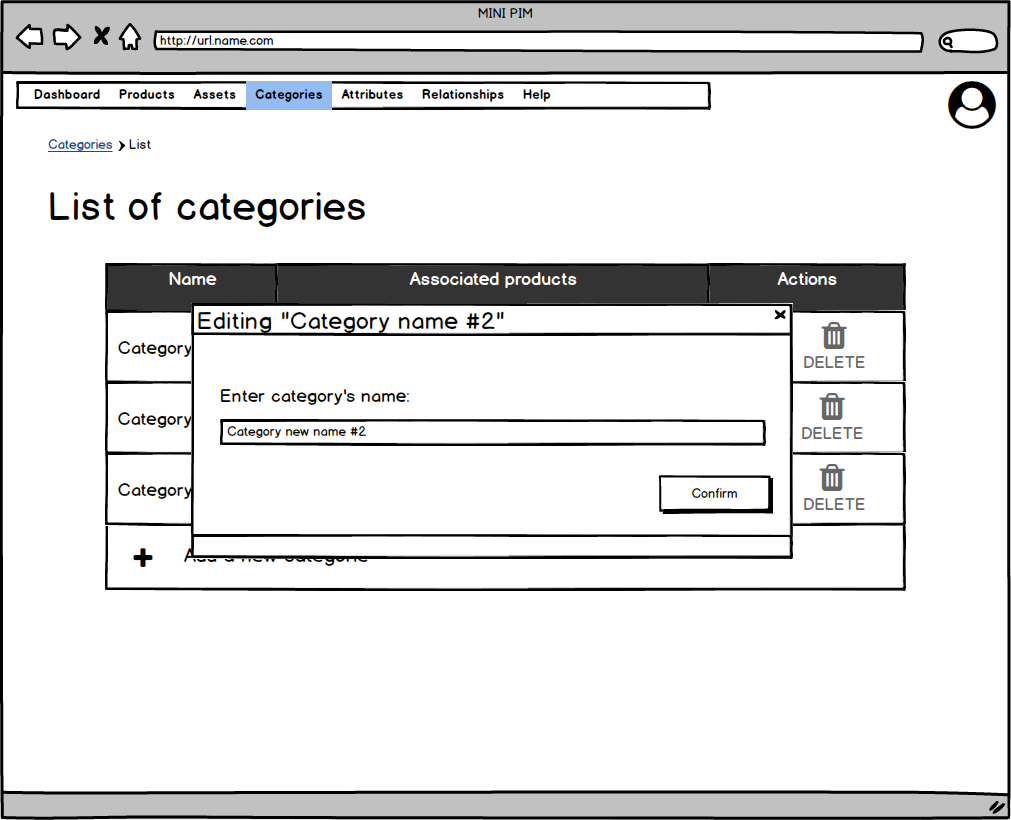
\includegraphics[width=1\linewidth]{mockups/RF4.3_1.png}
    \caption{Editar el nombre de relación}
   \end{figure}
\vspace{1.0cm}

\begin{figure}[H]
    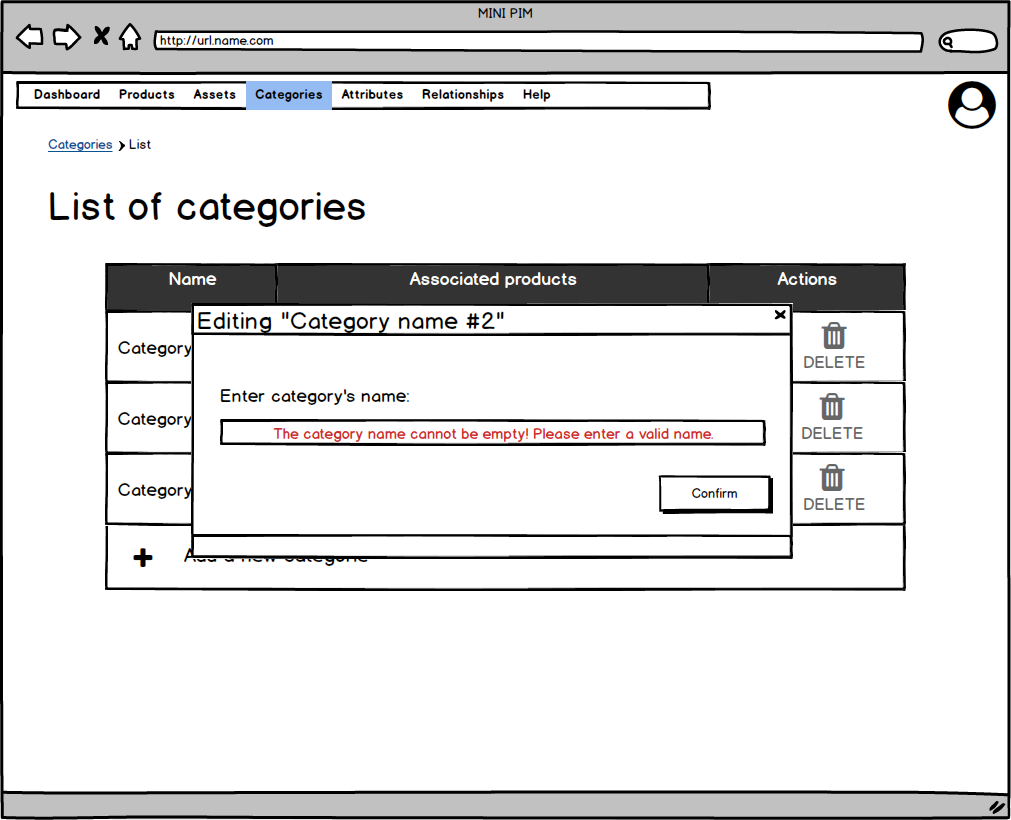
\includegraphics[width=1\linewidth]{mockups/RF4.3_2.png}
    \caption{Error por dejar el nombre vacío}
   \end{figure}
\vspace{1.0cm}

\newpage % Nuevo caso de uso en nueva página